\documentclass{beamer}

\mode<presentation> {


\usetheme{Madrid}



%\setbeamertemplate{footline} % To remove the footer line in all slides uncomment this line
\setbeamertemplate{footline}[page number] % To replace the footer line in all slides with a simple slide count uncomment this line

\setbeamertemplate{navigation symbols}{} % To remove the navigation symbols from the bottom of all slides uncomment this line
}

\usepackage{graphicx} % Allows including images
\usepackage{booktabs} % Allows the use of \toprule, \midrule and \bottomrule in tables
%\usepackage {tikz}
\usepackage{tkz-graph}
\GraphInit[vstyle = Shade]
\tikzset{
  LabelStyle/.style = { rectangle, rounded corners, draw,
                        minimum width = 2em, fill = yellow!50,
                        text = red, font = \bfseries },
  VertexStyle/.append style = { inner sep=5pt,
                                font = \normalsize\bfseries},
  EdgeStyle/.append style = {->, bend left} }
\usetikzlibrary {positioning}
%\usepackage {xcolor}
\definecolor {processblue}{cmyk}{0.96,0,0,0}


\AtBeginSection[]{
  \begin{frame}
  \vfill
  \centering
  \begin{beamercolorbox}[sep=8pt,center,shadow=true,rounded=true]{title}
    \usebeamerfont{title}\insertsectionhead\par%
  \end{beamercolorbox}
  \vfill
  \end{frame}
}

% \setbeamerfont{bibliography item}{size=5pt}
% \setbeamerfont{bibliography entry author}{size=5pt}
% \setbeamerfont{bibliography entry title}{size=5pt}
% \setbeamerfont{bibliography entry location}{size=5pt}
% \setbeamerfont{bibliography entry note}{size=5pt}

\title[Short title]{Improving the performance of a Lattice Boltzmann fluid solver using TensorFlow}

\author{Vikram Singh}
\institute{The Perse School, Cambridge \\ Project conducted at University of  Cambridge Research Computing Services}
\date{August 23, 2019}

\begin{document}

\begin{frame}
\titlepage
\end{frame}

\begin{frame}{The Lattice Boltzmann Method}

\begin{itemize}
    \item Macroscopic variables \\  
    $\rho = \sum{f_\text{in}}$ \\
    $E(i,\rho,u) = \rho t_i (1+u + {u^2 \over 2} - {3|u|^2\over2})$
    \item Collision \\
    $f_\text{out} = f_\text{in} - \omega(f_\text{in}-E)$
    \item Streaming
    \item Boundary Conditions
    
\end{itemize}

\end{frame}

\begin{frame}{Tensorflow}

\begin{itemize}
    \item Used primarily in machine learning
    \item Efficient large array operations
    \item Parallelisable
\end{itemize}

\end{frame}

\begin{frame}{Implementation and Testing}

\begin{itemize}
    \item Implemented two D2Q9 Lattice Boltzmann solvers: 
    \begin{itemize}
        \item Using only Numpy
        \item Using TensorFlow for all lattice calculations
    \end{itemize}
    \vspace{10pt}
    \item Performed the following simulations with both solvers:
    \begin{enumerate}
        \item Flow around a cylinder with low viscosity ($420\times180$ lattice points)
        \item Flow around a cylinder with high viscosity ($420\times180$ lattice points)
        \item Flow around an airfoil ($420\times180$ lattice points)
        \item Flow through a narrowing pipe ($420\times180$ lattice points)
        \item Flow through a bending pipe ($1000\times452$ lattice points)
        \item Flow in a lid driven cavity ($180\times180$ lattice points)
    \end{enumerate}
    \vspace{30pt}
    \item \small\url{github.com/vikram8128/PythonLatticeBoltzmann}
\end{itemize}

\end{frame}


\begin{frame}{Simulations}

% Explain Numpy, TF versions

\begin{figure}[H] 
	\centering
	\label{videoCuts}
	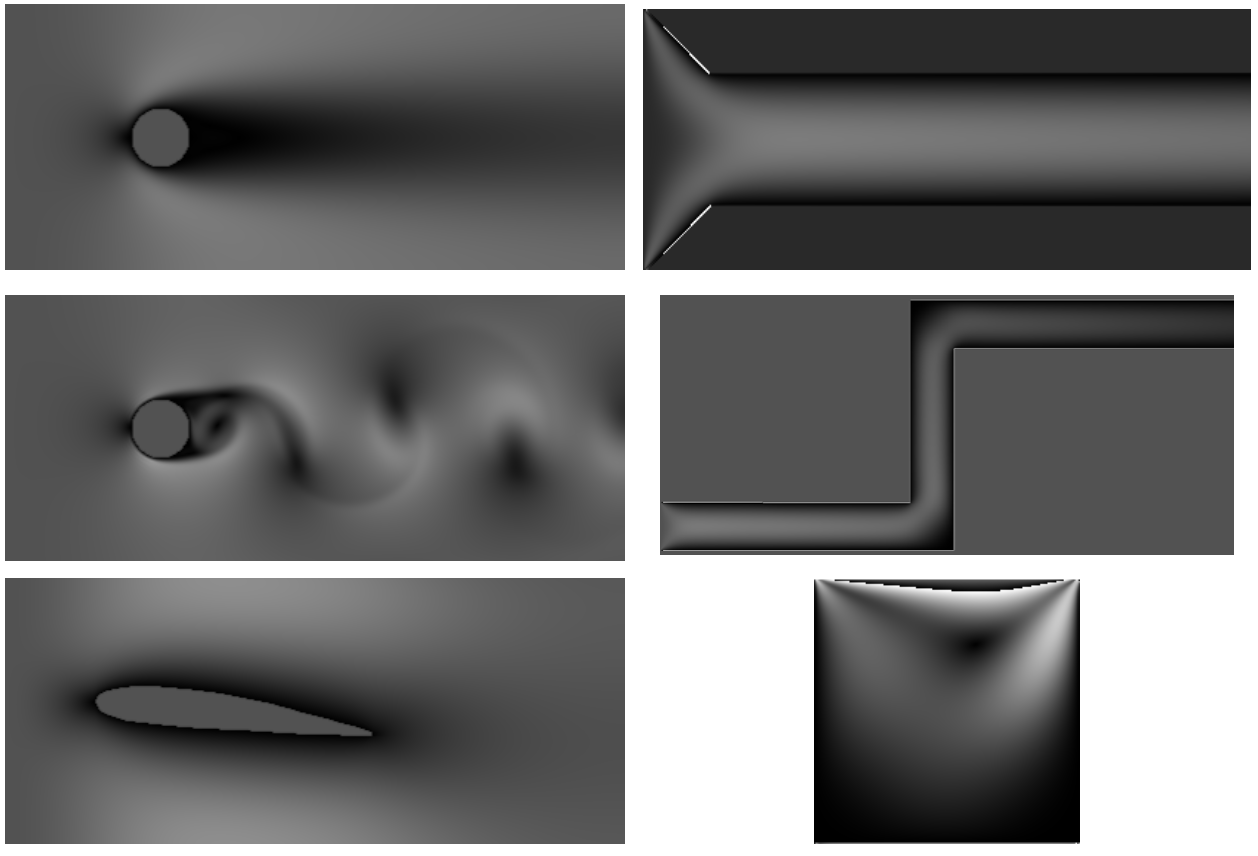
\includegraphics[width=4.5in]{Diagrams/SimulationSamples.png}
\end{figure}

\end{frame}

\begin{frame}{Animations}

\end{frame}

\begin{frame}{Results}


\begin{figure}[H] 
	\centering
	\label{videoCuts}
	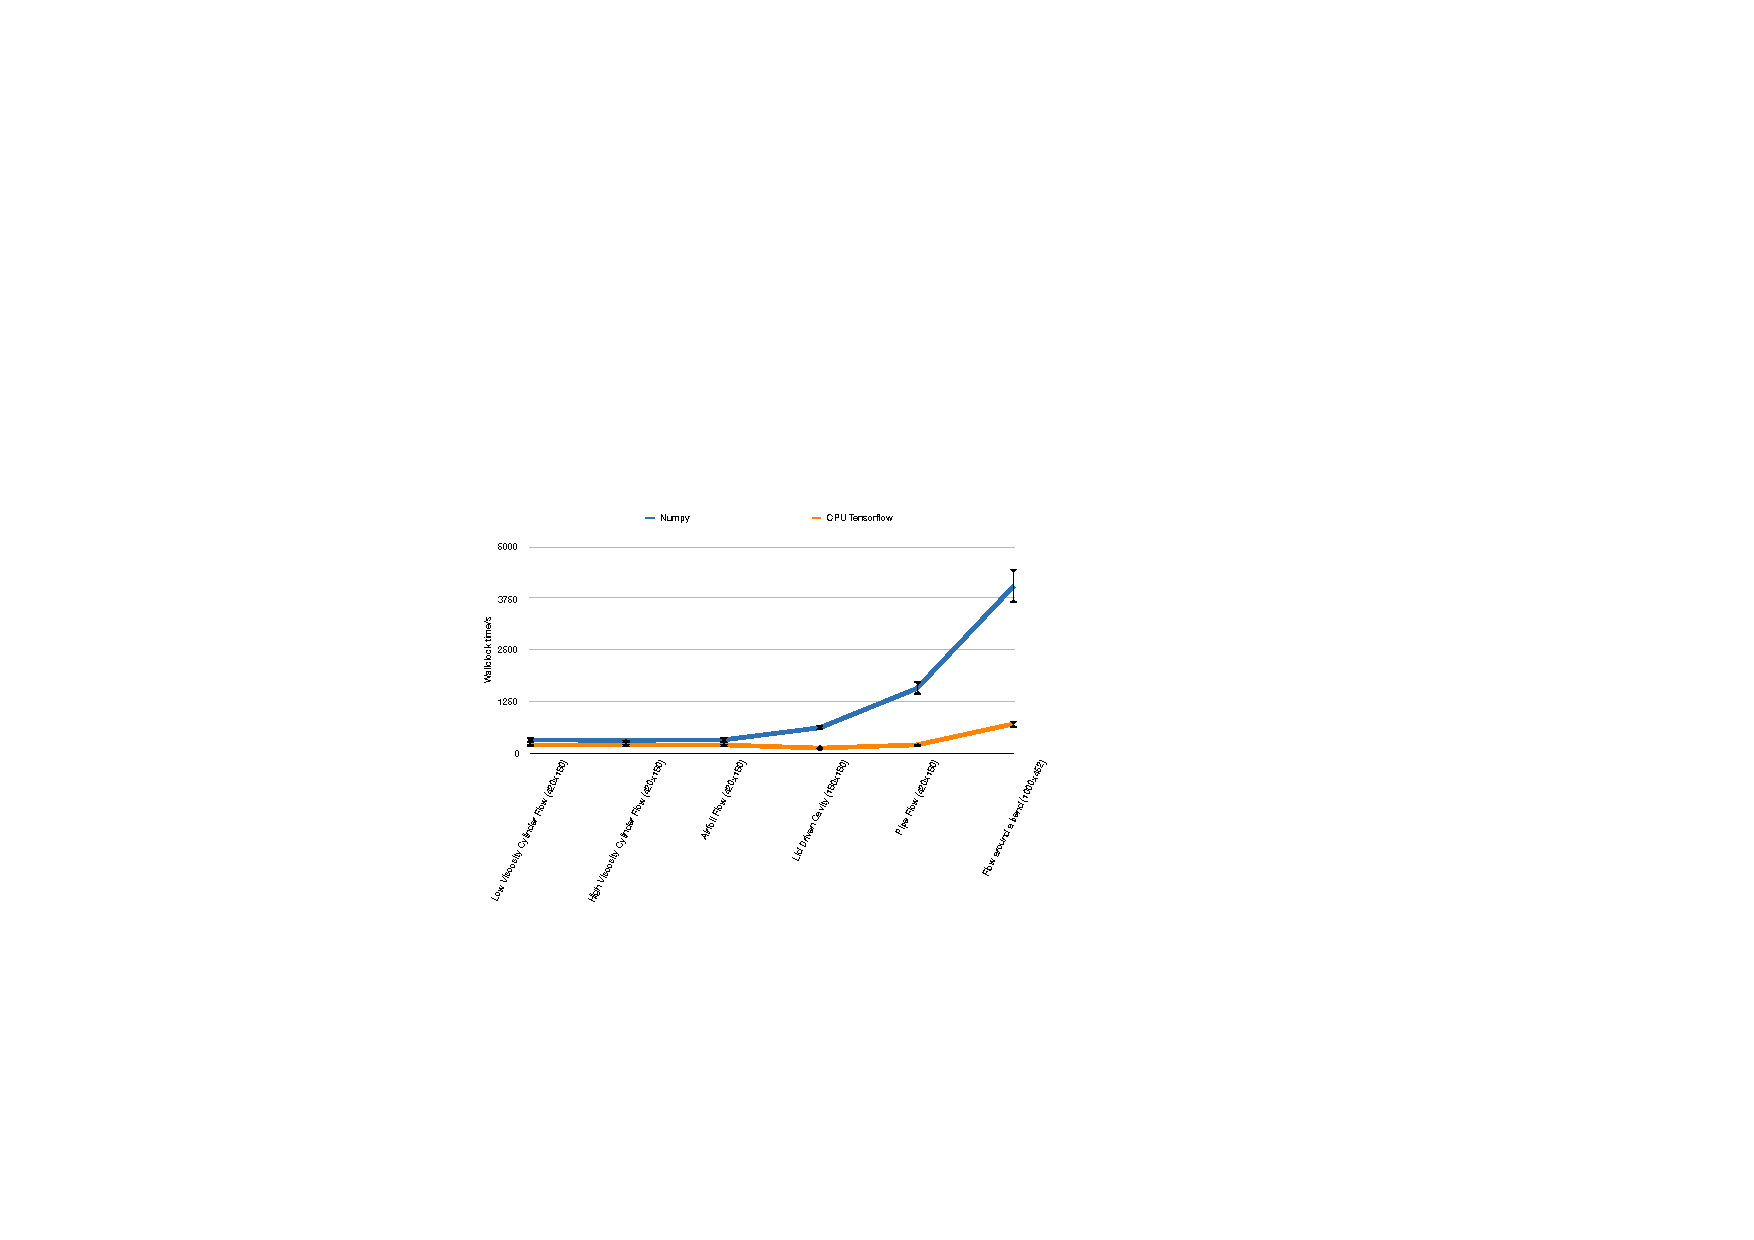
\includegraphics[width=4.5in]{Diagrams/TimeGraph.pdf}
\end{figure}

\end{frame}

\begin{frame}{Results}

\begin{table}[H]
\caption{Wallclock times in seconds taken by each simulation}
\begin{center}
\begin{tabular}{c||c|c|c|c|c|c}
\emph{Simulation} & 1 & 2 & 3 & 4 & 5 & 6\\
\hline
\hline
\emph{Numpy} & 316 & 311 & 319 & 1565 & 4043 & 615 \\
\hline
\emph{TensorFlow} & 198 & 198 & 198 & 199 & 708 & 122 \\
\hline
\end{tabular}
\end{center}
\end{table}

\end{frame}

\begin{frame}{Results}

\begin{figure}[H] 
	\centering
	\label{videoCuts}
	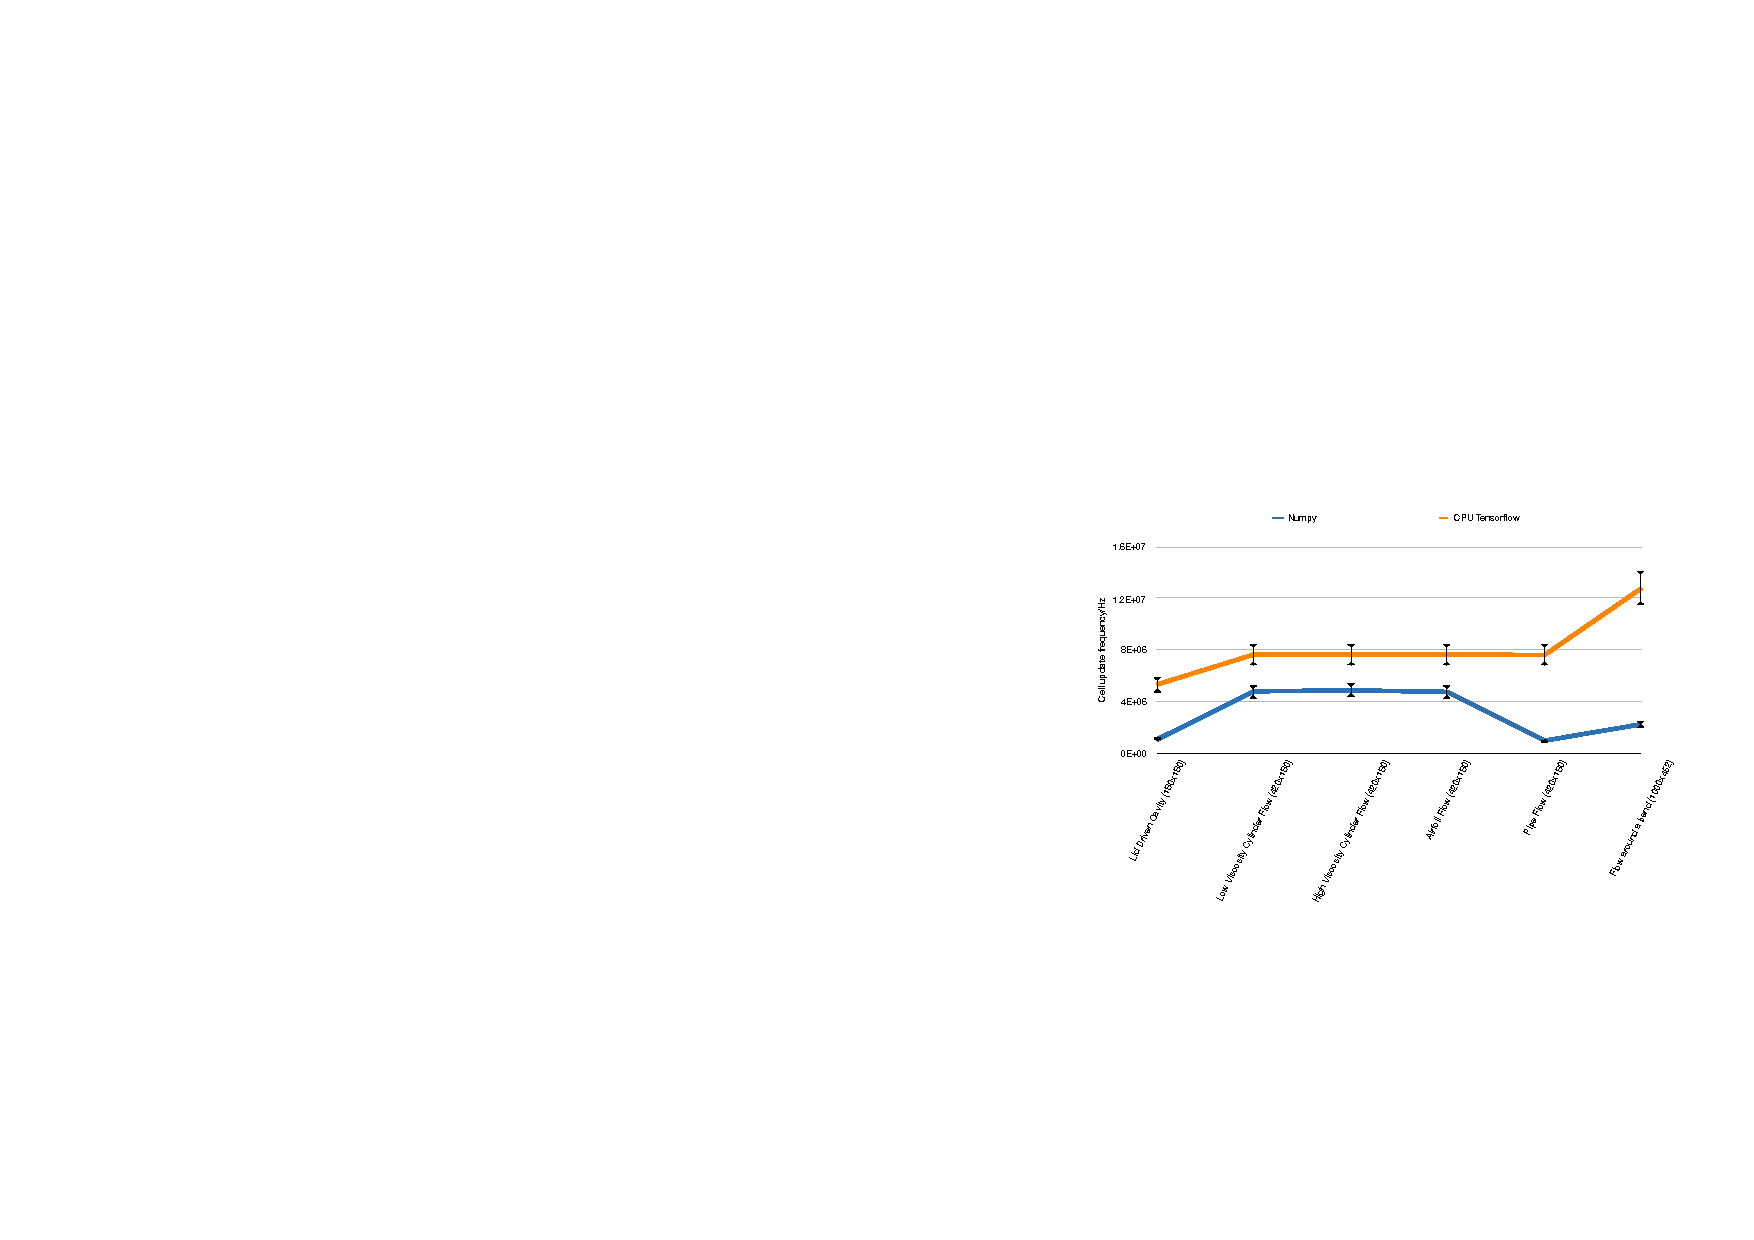
\includegraphics[width=4.5in]{Diagrams/FreqGraph.pdf}
\end{figure}

\end{frame}

\begin{frame}{Results}

\begin{table}[H]
\caption{Cell updates per second (MHz) for each of the simulations}
\begin{center}
\begin{tabular}{c||c|c|c|c|c|c}
\emph{Simulation} & 1 & 2 & 3 & 4 & 5 & 6\\
\hline
\hline
\emph{Numpy} & 4.78 & 4.86 & 4.74 & 0.966 & 2.24 & 1.05 \\
\hline
\emph{TensorFlow} & 7.64 & 7.64 & 7.64 & 7.60 & 12.8 & 5.31 \\
\hline
\end{tabular}
\end{center}
\end{table}

\end{frame}

\begin{frame}{Conclusions}

\begin{itemize}
    \item Tensorflow outperforms Numpy in all simulations
    \item Improvement scales well with size and obstacle complexity
\end{itemize}

\end{frame}

\begin{frame}{Further Work}

\begin{itemize}
    \item Expanding to 3D
    \item Using GPU Tensorflow
\end{itemize}

\end{frame}


\begin{frame}{Thank you}

\begin{itemize}
    \item Thank you very much to Jeffrey for suggesting this project and supervising my work.
    \item Thank you for listening.
\end{itemize}

\end{frame}


\begin{frame}{References}

\begin{thebibliography}{}\tiny

\bibitem{LBPaper} Chen, Shiyi, Doolen, Gary D. (1998). \emph{LATTICE BOLTZMANN METHOD FOR FLUID FLOWS} Annual Review of Fluid Mechanics 30 (1): 329–364 doi:10.1146/annurev.fluid.30.1.329

\bibitem{LBBook} Alexander J. Wagner (2008) \emph{A Practical Introduction to the Lattice Boltzmann Method}, North Dakota State University

\bibitem{TFDocs} TensorFlow Documentation (\url{www.tensorflow.org/api_docs/python/})

\end{thebibliography}

\end{frame}


\end{document}

